% Options for packages loaded elsewhere
\PassOptionsToPackage{unicode}{hyperref}
\PassOptionsToPackage{hyphens}{url}
\PassOptionsToPackage{dvipsnames,svgnames,x11names}{xcolor}
%
\documentclass[
  english,
]{article}
\usepackage{amsmath,amssymb}
\usepackage{lmodern}
\usepackage{setspace}
\usepackage{iftex}
\ifPDFTeX
  \usepackage[T1]{fontenc}
  \usepackage[utf8]{inputenc}
  \usepackage{textcomp} % provide euro and other symbols
\else % if luatex or xetex
  \usepackage{unicode-math}
  \defaultfontfeatures{Scale=MatchLowercase}
  \defaultfontfeatures[\rmfamily]{Ligatures=TeX,Scale=1}
\fi
% Use upquote if available, for straight quotes in verbatim environments
\IfFileExists{upquote.sty}{\usepackage{upquote}}{}
\IfFileExists{microtype.sty}{% use microtype if available
  \usepackage[]{microtype}
  \UseMicrotypeSet[protrusion]{basicmath} % disable protrusion for tt fonts
}{}
\makeatletter
\@ifundefined{KOMAClassName}{% if non-KOMA class
  \IfFileExists{parskip.sty}{%
    \usepackage{parskip}
  }{% else
    \setlength{\parindent}{0pt}
    \setlength{\parskip}{6pt plus 2pt minus 1pt}}
}{% if KOMA class
  \KOMAoptions{parskip=half}}
\makeatother
\usepackage{xcolor}
\IfFileExists{xurl.sty}{\usepackage{xurl}}{} % add URL line breaks if available
\IfFileExists{bookmark.sty}{\usepackage{bookmark}}{\usepackage{hyperref}}
\hypersetup{
  pdflang={en},
  colorlinks=true,
  linkcolor={blue},
  filecolor={Maroon},
  citecolor={blue},
  urlcolor={blue},
  pdfcreator={LaTeX via pandoc}}
\urlstyle{same} % disable monospaced font for URLs
\usepackage[margin=1.25in]{geometry}
\usepackage{longtable,booktabs,array}
\usepackage{calc} % for calculating minipage widths
% Correct order of tables after \paragraph or \subparagraph
\usepackage{etoolbox}
\makeatletter
\patchcmd\longtable{\par}{\if@noskipsec\mbox{}\fi\par}{}{}
\makeatother
% Allow footnotes in longtable head/foot
\usepackage{footnote} % For some unknown reason, footnotehyper clashes with French
\makesavenoteenv{longtable}
\usepackage{graphicx}
\makeatletter
\def\maxwidth{\ifdim\Gin@nat@width>\linewidth\linewidth\else\Gin@nat@width\fi}
\def\maxheight{\ifdim\Gin@nat@height>\textheight\textheight\else\Gin@nat@height\fi}
\makeatother
% Scale images if necessary, so that they will not overflow the page
% margins by default, and it is still possible to overwrite the defaults
% using explicit options in \includegraphics[width, height, ...]{}
\setkeys{Gin}{width=\maxwidth,height=\maxheight,keepaspectratio}
% Set default figure placement to htbp
\makeatletter
\def\fps@figure{htbp}
\makeatother
\setlength{\emergencystretch}{3em} % prevent overfull lines
\providecommand{\tightlist}{%
  \setlength{\itemsep}{0pt}\setlength{\parskip}{0pt}}
\setcounter{secnumdepth}{-\maxdimen} % remove section numbering
\newlength{\cslhangindent}
\setlength{\cslhangindent}{1.5em}
\newlength{\csllabelwidth}
\setlength{\csllabelwidth}{3em}
\newlength{\cslentryspacingunit} % times entry-spacing
\setlength{\cslentryspacingunit}{\parskip}
\newenvironment{CSLReferences}[2] % #1 hanging-ident, #2 entry spacing
 {% dont indent paragraphs
  \setlength{\parindent}{0pt}
  % turn on hanging indent if param 1 is 1
  \ifodd #1
  \let\oldpar\par
  \def\par{\hangindent=\cslhangindent\oldpar}
  \fi
  % set entry spacing
  \setlength{\parskip}{#2\cslentryspacingunit}
 }%
 {}
\usepackage{calc}
\newcommand{\CSLBlock}[1]{#1\hfill\break}
\newcommand{\CSLLeftMargin}[1]{\parbox[t]{\csllabelwidth}{#1}}
\newcommand{\CSLRightInline}[1]{\parbox[t]{\linewidth - \csllabelwidth}{#1}\break}
\newcommand{\CSLIndent}[1]{\hspace{\cslhangindent}#1}

%%%%%%%% START HEADER PARTIAL %%%%%%%%%%%%

% Formatting of tables & knitr::kable and kableExtra functionality
\usepackage{float}
\usepackage{colortbl}
\usepackage{pdflscape}
\usepackage{tabu}
\usepackage{threeparttable}

% Line numbering

% endfloat stuff

% fancyhdr pagestyle

% Environment for keywords
\makeatletter
\newcommand\keywordsname{Keywords}
\newenvironment*{keywords}[1][\keywordsname]{\if@twocolumn \else \small \quotation \fi \begin{center} \textbf{\textit{#1} \\}}{\end{center}\if@twocolumn \else \small \endquotation \fi}
\newenvironment*{keywordsinline}[1][\keywordsname]{\if@twocolumn \else \small \quotation \fi \begin{center} \textbf{\textit{#1}: }}{\end{center}\if@twocolumn \else \small \endquotation \fi}
\makeatother

% Environment for abstract that takes new abstract name
\newenvironment{renameableabstract}[1][\abstractname]{\let\oldabstractname\abstractname \renewcommand{\abstractname}{#1} \begin{abstract}}{\end{abstract} \renewcommand{\abstractname}{\oldabstractname}}

%%%%%%%% END HEADER PARTIAL %%%%%%%%%%%%

\usepackage{tikz}
\usetikzlibrary{angles,positioning,arrows.meta, quotes, shapes, shapes.geometric}
\usepackage{graphicx}
\usepackage{emoji}
\usepackage{caption, subcaption}
\usepackage{booktabs}
\usepackage{longtable}
\usepackage{array}
\usepackage{multirow}
\usepackage{wrapfig}
\usepackage{float}
\usepackage{colortbl}
\usepackage{pdflscape}
\usepackage{tabu}
\usepackage{threeparttable}
\usepackage{threeparttablex}
\usepackage[normalem]{ulem}
\usepackage{makecell}
\usepackage{xcolor}
\ifXeTeX
  % Load polyglossia as late as possible: uses bidi with RTL langages (e.g. Hebrew, Arabic)
  \usepackage{polyglossia}
  \setmainlanguage[]{}
\else
  \usepackage[english,main=english]{babel}
% get rid of language-specific shorthands (see #6817):
\let\LanguageShortHands\languageshorthands
\def\languageshorthands#1{}
\fi
\ifLuaTeX
  \usepackage{selnolig}  % disable illegal ligatures
\fi

\title{Interaction structure constrains\\
the emergence of conventions in group communication}

%%%%%%% START AUTHOR PARTIAL %%%%%%%%%%%%%%%

%%%%% Authors, affiliations and author notes stuff %%%%%

% Macros for creating and referencing stored reference
\makeatletter
\def\MyNewLabel#1#2#3{\expandafter\gdef\csname #1@#2\endcsname{#3}}

\def\MyRef#1#2{\@ifundefined{#1@#2}{???}{\csname #1@#2\endcsname}}

\newcommand*\ifcounter[1]{%
  \ifcsname c@#1\endcsname
    \expandafter\@firstoftwo
  \else
    \expandafter\@secondoftwo
  \fi
}
\makeatother

% Create labels for Addresses if the are given by code
\MyNewLabel{ADDRTXT}{Stanford}{Stanford University}
\MyNewLabel{ADDRTXT}{UW-Madison}{University of Wisconsin -- Madison}

% Create labels for Footnotes if they are given by code
\MyNewLabel{ANOTETXT}{corresp}{Corresponding author. Email: \href{mailto:vboyce@stanford.edu}{\nolinkurl{vboyce@stanford.edu}}}

%%% Special footnotes for addresses and author footnotes
\usepackage{bigfoot}
\DeclareNewFootnote{Addr}[arabic] % Only used for NOT authblk
\DeclareNewFootnote{ANote}[fnsymbol]

%%% Address and author notes as a function of format %%%
 % Use authblk for affiliations %%%%%%%%%%%
\usepackage{authblk}

% Always separate by commas
\renewcommand\Authsep{, }
\renewcommand\Authand{, }
\renewcommand\Authands{, }

% Counter for addresses and footnotes
\newcounter{addrcnt}

% thanks definition that doesnt produce superscript marks
\makeatletter
\newcommand*\createaddrlblbycode[1]{%
  \ifcounter{ADDRLBL@#1}
    {}
    {\refstepcounter{addrcnt}\newcounter{ADDRLBL@#1}\setcounter{ADDRLBL@#1}{\value{addrcnt}}}%
}

\newcommand*\addrlblbycode[1]{\arabic{ADDRLBL@#1}}

\newcommand*\addrbycode[1]{%
  \ifcounter{ADDR@#1}
    {}
    {\newcounter{ADDR@#1}%
     \affil[\addrlblbycode{#1}]{\MyRef{ADDRTXT}{#1}}}%
}

\newcommand*\createanotelblbycode[1]{%
  \ifcounter{ANOTELBL@#1}
    {}
    {\refstepcounter{footnoteANote}\newcounter{ANOTELBL@#1}\setcounter{ANOTELBL@#1}{\value{footnoteANote}}}%
}

\newcommand*\anotelblbycode[1]{\fnsymbol{ANOTELBL@#1}}

\newcommand*\anotebycode[1]{%
  \ifcounter{ANOTE@#1}
    {}
    {\newcounter{ANOTE@#1}%
     \footnotetextANote[\value{ANOTELBL@#1}]{\MyRef{ANOTETXT}{#1}}}%
}
\makeatother


\createaddrlblbycode{Stanford}


\createanotelblbycode{corresp}

\author[%
\addrlblbycode{Stanford}%
,%
$\anotelblbycode{corresp}$%
]{Veronica Boyce}

\addrbycode{Stanford}


\createaddrlblbycode{UW-Madison}



\author[%
\addrlblbycode{UW-Madison}%
]{Robert D. Hawkins}

\addrbycode{UW-Madison}


\createaddrlblbycode{Stanford}



\author[%
\addrlblbycode{Stanford}%
]{Noah D. Goodman}

\addrbycode{Stanford}


\createaddrlblbycode{Stanford}



\author[%
\addrlblbycode{Stanford}%
]{Michael C. Frank}

\addrbycode{Stanford}


%endif(authblk)

%%%%%%%%% END AUTHOR PARTIAL %%%%%%%%

\date{}

\begin{document}
\maketitle

%%%%%%%%%% START AFTER TITLE PARTIAL %%%%%%%%%%%%%
\anotebycode{corresp}


%%%%%%%%%% END AFTER TITLE PARTIAL %%%%%%%%%%%%%


\setstretch{1}
\begin{otherlanguage}{english}

\begin{abstract}
Real-world communication frequently requires language producers to address more than one comprehender at once, yet most psycholinguistic research focuses on one-on-one communication.
As the audience size grows, interlocuters face new challenges that do not arise in dyads.
They must consider multiple perspectives and weigh multiple sources of feedback to build shared understanding.
Here, we ask which properties of the group's \emph{interaction structure} facilitate successful communication.
We used a repeated reference game paradigm in which directors instructed between one and five matchers to choose specific targets out of a set of abstract figures.
Across 313 games (\(N=1,319\) participants), we manipulated several key constraints on the group's interaction, including the amount of feedback that matchers could give to directors and the availability of peer interaction between matchers.
Across groups of different sizes and interaction constraints, describers produced increasingly efficient utterances and matchers made increasingly accurate selections.
Critically, however, we found that smaller groups and groups with less-constrained interaction structures (``thick channels'') showed stronger convergence to group-specific conventions than large groups with constrained interaction structures (``thin channels''), which struggled with convention formation.
Overall, these results shed new light on the core structural factors that enable communication to thrive in larger groups.

\end{abstract}

\end{otherlanguage}

\hypertarget{introduction}{%
\section{Introduction}\label{introduction}}

Much of human social life revolves around communication in groups.
At school, teachers address large classrooms of children (\protect\hyperlink{ref-cazden1988classroom}{Cazden 1988}); at home, we chat with groups of friends and family members over dinner (\protect\hyperlink{ref-tannen2005conversational}{Tannen 2005}); and at work, we attend meetings with colleagues and managers (\protect\hyperlink{ref-caplow1957organizational}{Caplow 1957}, \protect\hyperlink{ref-zack1993interactivity}{Zack 1993}).
Such settings present considerable challenges that do not arise in the purely two-party (dyadic) settings typically studied in psychology (\protect\hyperlink{ref-traum2004}{Traum 2004}, \protect\hyperlink{ref-ginzburg2005}{Ginzburg \& Fernandez 2005}, \protect\hyperlink{ref-branigan2006}{Branigan 2006}).
For example, producers need to account for the fact that different comprehenders in the group may have different mental states or levels of background understanding (\protect\hyperlink{ref-horton2002}{Horton \& Gerrig 2002}, \protect\hyperlink{ref-weber2003}{Weber \& Camerer 2003}, \protect\hyperlink{ref-horton2005}{Horton \& Gerrig 2005}, \protect\hyperlink{ref-fox-tree2013}{Fox Tree \& Clark 2013}, \protect\hyperlink{ref-yoon2014}{Yoon \& Brown-Schmidt 2014}, \protect\hyperlink{ref-yoon2018}{2018}), while comprehenders must account for the fact that utterances are not necessarily tailored to them (\protect\hyperlink{ref-carletta1998}{Carletta et al. 1998}, \protect\hyperlink{ref-fay2000}{Fay et al. 2000}, \protect\hyperlink{ref-metzing2003}{Metzing \& Brennan 2003}, \protect\hyperlink{ref-rogers2013}{Rogers et al. 2013}, \protect\hyperlink{ref-tolins2016}{Tolins \& Fox Tree 2016}, \protect\hyperlink{ref-cohngordon}{Cohn-Gordon et al. 2019}, \protect\hyperlink{ref-yoon2019}{Yoon \& Brown‐Schmidt 2019}).
What enables producers and comprehenders to nevertheless overcome these challenges and navigate multi-party settings with relative ease?

One promising set of hypotheses centers on the group's \emph{interaction structure}, the set of constraints placed on the group's shared communication channel.
Many different aspects of interaction structure have been implicated in the effectiveness of dyadic communication, including the availability and quality of concurrent feedback (\protect\hyperlink{ref-krauss1966}{Krauss \& Weinheimer 1966}, \protect\hyperlink{ref-KraussBricker67_Delay}{Krauss \& Bricker 1967}, \protect\hyperlink{ref-kraut1982listener}{Kraut et al. 1982}), the bandwidth of the communication modality (\protect\hyperlink{ref-dewhirst1971influence}{Dewhirst 1971}, \protect\hyperlink{ref-KraussEtAl77}{Krauss et al. 1977}), and the group's access to a shared workspace (\protect\hyperlink{ref-clark2004speaking}{Clark \& Krych 2004}, \protect\hyperlink{ref-garrod2007foundations}{Garrod et al. 2007}).
Yet larger groups introduce qualitatively different dimensions of interaction structure, leading to a large but often inconsistent body of findings even for these well-understood factors (\protect\hyperlink{ref-hiltz1986experiments}{Hiltz et al. 1986}, \protect\hyperlink{ref-swaab2012communication}{Swaab et al. 2012}).
While communication is generally expected to deteriorate as groups get larger (\protect\hyperlink{ref-seaman1997communication}{Seaman \& Basili 1997}, \protect\hyperlink{ref-macmillan_communication_2004}{MacMillan et al. 2004}), the structural ``thickness'' of the feedback channel may slow such deterioration (\protect\hyperlink{ref-ahern1994effect}{Ahern 1994}, \protect\hyperlink{ref-parisi2005evaluating}{Parisi \& Brungart 2005}).

In this paper, we develop an experimental paradigm for evaluating the relative contribution of these factors: a \emph{multi-party repeated reference game.}
The ability to distinguish one particular entity from other possible entities, known as \emph{reference}, is one of the most primitive and ubiquitous functions of communication.
Reference games (\protect\hyperlink{ref-Wittgenstein1953}{Wittgenstein 1953}, \protect\hyperlink{ref-lewis1969convention}{Lewis 1969}) have been widely used to study dyadic communication under controlled conditions in the lab.
They provide a clear metric of communicative effectiveness: how many words are required before a matcher successfully chooses a target image from a context of distractors?
\emph{Repeated} reference games, where the same target images appear multiple times in succession, were introduced to examine how interlocutors establish shared reference in the absence of conventional labels (\protect\hyperlink{ref-krauss1964}{Krauss \& Weinheimer 1964}, \protect\hyperlink{ref-clark1986}{Clark \& Wilkes-Gibbs 1986}).
At the beginning of the game, long and costly descriptions are typically required to succeed.
A key finding, however, is that dyads become increasingly efficient over the course of interaction.
Fewer words are required to achieve the same accuracy, but referring expressions also become more impenetrable to outsiders (\protect\hyperlink{ref-schober1989}{Schober \& Clark 1989}, \protect\hyperlink{ref-wilkes1992coordinating}{Wilkes-Gibbs \& Clark 1992}).
The evolution of referring expressions over repetitions shows the characteristic dynamics of conventions: \emph{stability}, or convergence on labels within a group, and \emph{arbitrariness}, or divergence to different across groups, suggesting that dyads leverage their shared communication history to coordinate on expectations about how to label the target images (\protect\hyperlink{ref-hawkins2023partners}{Hawkins et al. 2023}).

In principle, repeated reference games provide a strong operationalization of communicative effectiveness for the problem of multi-party communication: describers must simultaneously achieve shared reference with multiple matchers.
However, empirically studying multi-party communication raises a number of difficulties in practice.
A much larger pool of participants must be recruited to achieve sufficient power at the relevant unit of analysis -- the group -- spanning a very high-dimensional space of possible parameter settings (\protect\hyperlink{ref-almaatouq2022}{Almaatouq et al. 2022}).
We address this problem by drawing on recent technical advances that have made it newly possible to achieve such samples using interactive web-based platforms (\protect\hyperlink{ref-haber2019}{Haber et al. 2019}, \protect\hyperlink{ref-almaatouq2020empirica}{Almaatouq et al. 2021}, \protect\hyperlink{ref-hawkins2023partners}{Hawkins et al. 2023}).
Repeated reference games in web-based platforms have previously replicated earlier results from face-to-face studies (\protect\hyperlink{ref-hawkins2020}{Hawkins et al. 2020}), and arguably more closely resemble the interfaces used by modern teams who increasingly communicate through group text threads or popular platforms like Slack or Discord.

We leverage our platform to explore effects of group size and interaction channel thickness in a series of three experiments.
While we find that small groups reliably converge on group-specific ``shorthand'' regardless of the interaction structure, larger groups require thicker channels -- richer conversational feedback among members -- to achieve the same degree of coherence.
Thus, increasing group size alone does not impede communication; rather, larger groups may require stronger social and linguistic cues to establish common ground among all members.
More broadly, our work suggests that studying communication in larger groups is necessary to unveil critical aspects of interaction structure that have not been evident in typical dyadic settings.

\begin{figure*}[t!]

{\centering 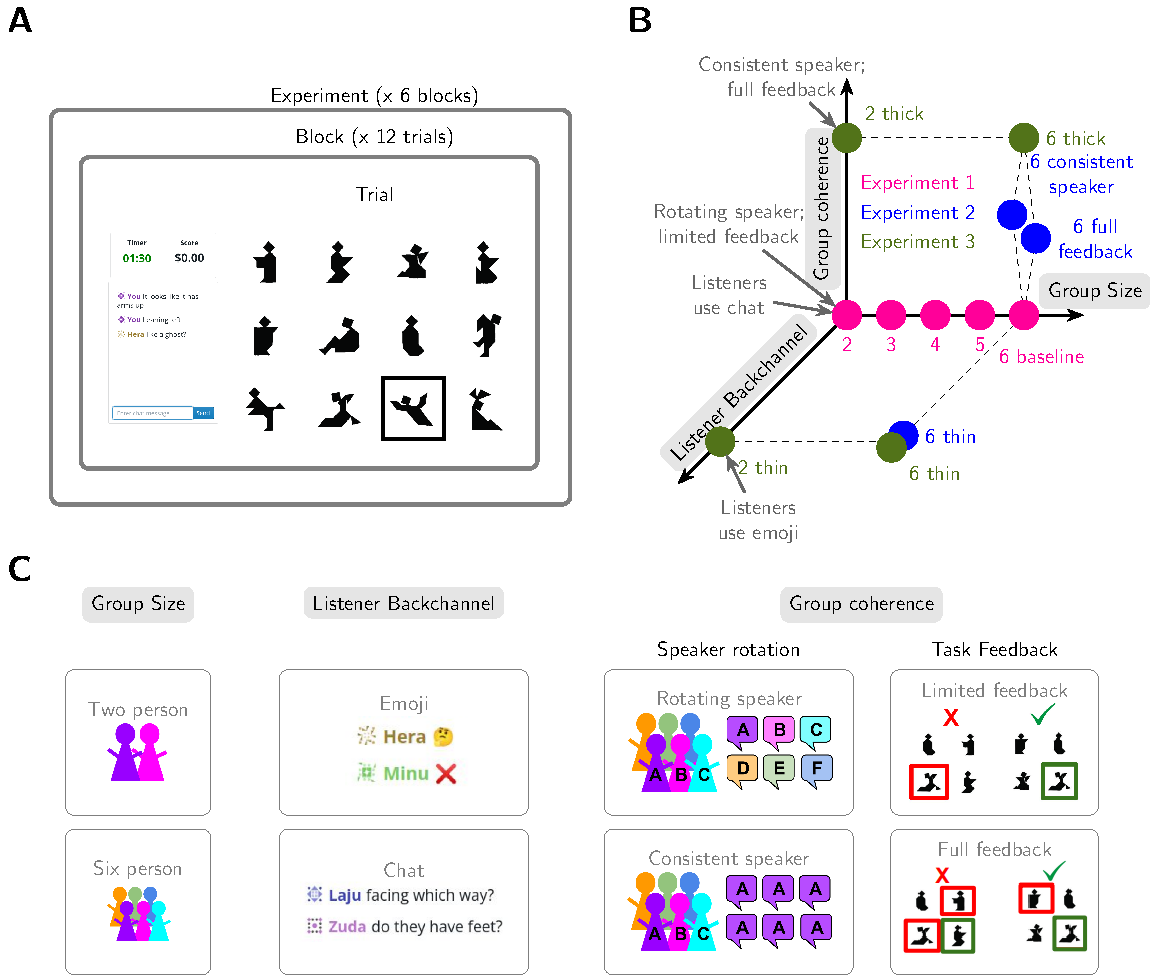
\includegraphics[width=1\linewidth]{expt-diagram3} 

}

\caption{(A) Participants played a repeated reference game in groups of size 2 to 6. On each trial, a describer described the target image to the group of matchers. Each image appeared once per block for six blocks. (B) Experiments varied along 3 dimensions: Group size, group coherence, and matcher backchannel. (C) Experiment 1 (pink) varied group size from 2 to 6 players while holding group coherence and backchannel constant. Experiment 2 (blue) held group size constant at 6 and manipulated the other dimensions. Experiment 3 (green) tested 4 corners of the space, crossing group size (2 vs. 6 players) with the thickness of interaction structure (high vs. low coherence and backchannel).}\label{fig:diagram}
\end{figure*}

\hypertarget{results}{%
\section{Results}\label{results}}

We recruited 1319 participants through Prolific, an online crowd-sourcing platform.
Participants were organized into 313 groups of size two to six for a communication game (Figure \ref{fig:behavioral}A).
On each trial, everyone in the group was shown a gallery of 12 tangram images (\protect\hyperlink{ref-clark1986}{Clark \& Wilkes-Gibbs 1986}, \protect\hyperlink{ref-hawkins2020}{Hawkins et al. 2020}, \protect\hyperlink{ref-ji2022abstract}{Ji et al. 2022}).
One player was designated the \emph{describer} and the others were designated the \emph{matchers}.
The describer was asked to use a chat box interface to describe a privately indicated \emph{target} image.
After all matchers guessed which of the 12 images was the target, they received task feedback and proceeded to the next trial.
The game consisted of 72 trials structured into 6 repetition blocks, where each image appeared as the target exactly once per block.

We manipulated the interaction structure of this game across 11 distinct conditions in 3 distinct pre-registered experiments (Figure \ref{fig:behavioral}B).
We systematically sampled points along four dimensions parameterizing different aspects of the interaction space.
We manipulated \emph{group size} (ranging from two to six), \emph{role stability} (whether or not participants took turns in the describer role), richness of \emph{task feedback} (whether or not matchers were able to see each other's responses), and richness of the \emph{matcher backchannel} (whether matchers were able to freely respond through a chatbox or could only use emojis; Figure \ref{fig:behavioral}C).
Other factors, such as the set of stimuli and background knowledge about one's partners, were held constant across games.

\hypertarget{overview-of-experiments}{%
\subsubsection{Overview of experiments}\label{overview-of-experiments}}

Experiment 1 began by investigating how performance scaled with group size.
Based on prior qualitative work, we predicted that larger groups face a more challenging coordination problem.
We continuously varied the number of players from 2 to 6 while keeping other factors constant.
For these conditions, the describer role rotated after each block, so that all players had at least one turn as describer.
Matchers had access to an unrestricted chat box, but only received binary task feedback about whether their individual selection was correct without revealing others' selections or the intended target.

Experiment 2 explored the role of interaction structure purely within the most challenging 6-player groups.
We manipulated two factors that we expected to increase group coherence and improve performance.
First, we maintained the same describer throughout rather than a rotating describer, such that the same individual has the opportunity to aggregate feedback across trials and track which matchers are struggling with which targets.
Second, we gave the group of matchers full feedback about what every other member of the group had selected, and we showed the intended target.
We also manipulated a factor that we expected to interfere with the ability to establish mutual understanding and thus impede performance.
In the limited backchannel condition, matchers were limited to four discrete emojis (green check, thinking face, red x, and laughing-crying face) that could convey simple valence and level of comprehension, but not any referential content.

Experiment 3 crossed the extremes of group size from experiment 1 (2 vs.~6 people) with the extremes of group interactions from Experiment 2 (\emph{thick} vs.~\emph{thin} interaction structure).
In the \emph{thick} condition, we maintained a consistent describer, gave all matchers full task feedback, and allowed them to freely use a chat box.
In the \emph{thin} condition, we forced the describer to rotate on each block, restricted feedback to their own binary correctness, and restricted the backchannel to the four emojis.
Note that the 2-player thick game most closely resembles the design of classic repeated reference games (\protect\hyperlink{ref-clark1986}{Clark \& Wilkes-Gibbs 1986}).

\begin{figure*}[t!]

{\centering \includegraphics[width=1\linewidth]{figs/behavioral-1} 

}

\caption{Behavioral results across all three experiments. (A-C). Matcher accuracy at selecting the target image. (D-F). Number of words produced by the describer each trial. For all, small dots are per game, per block means, and smooth lines are predictions from model fixed effects with 95\% credible intervals. Y-axes are truncated, and a few outliers points are not visible.}\label{fig:behavioral}
\end{figure*}

\hypertarget{smaller-and-higher-coherence-groups-are-more-accurate}{%
\subsubsection{Smaller and higher-coherence groups are more accurate}\label{smaller-and-higher-coherence-groups-are-more-accurate}}

Our first set of hypotheses focused on group performance: how accurately and efficiently groups were able to perform the referential task.
We characterize group performance along two complementary metrics: (1) matcher accuracy and (2) describer efficiency.
Matcher accuracy is given by the percent of matchers on each trial who successfully selected the target referent.
Describer efficiency is given by the number of words produced by the describer to achieve that degree of matcher accuracy in the group.
The degree to which describers are able to communicate more efficiently without negatively impacting matcher accuracy is indicative of convergence on a more effective shared communication protocol within the group.

We begin by examining matcher accuracy, the extent to which the intended target was reliably transmitted to all matchers.
We constructed a series of 5 logistic mixed-effects regression models predicting accuracy as a function of condition and repetition block (separate models were run for experiment 1, each condition in experiment 2, and experiment 3).
Across all conditions, we observed strong positive effects of repetition block, indicating improved performance over time (Figure \ref{fig:behavioral}A-C, SI Tables 4-8).
In Experiment 3, larger games began with lower initial accuracy (\(\beta=-0.64,\:95\%\:\mathrm{CrI}=[-1.05, -0.25]\)) and improved more slowly (\(\beta=-0.34,\:95\%\:\mathrm{CrI}=[-0.43, -0.25]\)) than smaller games, although group size differences were not reliable in Experiment 1 (SI Table 4).
Among large groups in Experiment 2, accuracy was higher in the thicker conditions than in the condition with thin interaction structure (SI Tables 5-7), although effects of game thickness were not reliable in Experiment 3 (SI Table 8).

Because each experiment only explored a slice of the full parameter space, we also considered an exploratory analysis that pooled data across experiments, aiming to mitigate the loss in power from running entirely separate regression models.
Specifically, we aggregated data from all experiments into a post-hoc mega-analytic model predicting accuracy as a function of repetition block, game thickness (thin v. not-thin) and game size.
Overall, we found evidence that accuracy increased over time (\(\beta=0.46,\:95\%\:\mathrm{CrI}=[0.4, 0.52]\)) but the rate of increase was reduced for thin games (\(\beta=-0.12,\:95\%\:\mathrm{CrI}=[-0.21, -0.02]\)) and larger games (\(\beta=-0.07,\:95\%\:\mathrm{CrI}=[-0.09, -0.05]\)) compared to smaller or thicker games.
That is, smaller groups and groups with higher coherence tended to be more accurate, though the magnitude and reliability of these effects varied across individual experiments.

\hypertarget{smaller-and-higher-coherence-groups-are-more-efficient}{%
\subsubsection{Smaller and higher-coherence groups are more efficient}\label{smaller-and-higher-coherence-groups-are-more-efficient}}

After establishing that groups were able to communicate accurately, we turned to the challenges faced by describers when deciding how much information to provide.
Specifically, we predicted that larger and more heterogeneous groups may initially require more information, but that thicker interaction structure may similarly allow describers to communicate more effectively over time.
We tested these predictions using linear mixed-effects models predicting the number of words a describer produced on each trial as a function of condition and block.
These models counted all words the describer produced, including after matcher contributions (similar effects were found in models predicting the length of describer's utterances before any matcher contributions, see SI Tables 19-22).

First, as predicted, describers in larger groups produced longer descriptions at the outset than describers in smaller groups (Figure \ref{fig:behavioral}D-F).
This effect held for the continuous manipulation of group size for Experiment 1 (\(\beta=1.6,\:95\%\:\mathrm{CrI}=[0.62, 2.6]\)) as well as the 2-person versus 6-person manipulation in Experiment 3 (\(\beta=7.51,\:95\%\:\mathrm{CrI}=[3.63, 11.3]\)).
Smaller groups also continued to use shorter descriptions than larger groups over the course of the game.
In Experiment 1, the rate at which efficiency increased was similar across different size groups (\(\beta=-0.09,\:95\%\:\mathrm{CrI}=[-0.37, 0.18]\)).
In Experiment 3, larger groups reduced faster than smaller ones (\(\beta=-1.22,\:95\%\:\mathrm{CrI}=[-2.06, -0.29]\)), but the faster reduction did not fully make up for the longer initial starting point.

While thin 6-person games showed a flatter reduction trajectory than thicker 6-person games in Experiment 2 (SI Tables 10-12), there was no reliable effect of game thickness on reduction in Experiment 3 (SI Table 13).
Aggregating across experiments with a mega-analytic model, however, suggested that larger games were associated with steeper reduction (\(\beta=-0.36,\:95\%\:\mathrm{CrI}=[-0.51, -0.2]\)) from a more verbose starting point (\(\beta=2.12,\:95\%\:\mathrm{CrI}=[1.5, 2.75]\)) than smaller games, and thin games had shallower reduction curves (\(\beta=0.79,\:95\%\:\mathrm{CrI}=[0.04, 1.52]\)) than thicker games.
Overall, then, smaller games used shorter descriptions than larger games across various time points in the experiment, and thinner games reduced less than thicker games.

\begin{table}
    \centering

    \caption{Examples from 6-player groups in Experiment 3 of successful descriptions for the same image across repetitions. Describers are indicated with an asterisk. More example descriptions are in SI Tables 1 and 2. \\\label{listener-examples}}
    \begin{subtable}{0.5\linewidth}
        \centering
            \begin{tabular}{lp{2.5in}}
            \hline
            
            \multicolumn{2}{c}{\textbf{6-person thick game}}\\
            \multicolumn{2}{l}{\textit{Rep 1: 4/5 correct}}\\
            A*  &   sitting down no legs showing   \\                
            C   & no arms?\\                       
            B  &    Bunny ears?  \\                                  
            A*  &   legs showing to one side no arms  \\             
            C  &    kinda like kneeling?  \\                         
            A*  &   no feet      \\                                  
            A*   &  yes kneeling  \\
            \multicolumn{2}{l}{\textit{Rep 2: 5/5 correct}}\\
            A*  &   sitting down with no feet showing. legs to one side \\
            A*  &  no arms   \\                                     
            E &      Swaddled up like a bb \\                         
            C  &    cute bb    \\                                    
            D  &    I think that's the one that looks like a ghost to me, like he's wearing a sheet. (?)\\
            \multicolumn{2}{l}{\textit{Rep 3: 5/5 correct}}\\
            A*  &    sitting down no arms showing legs to one side  \\
            E  &   the bb   \\                                      
            B  &  Swadled baby?  \\                                
            F &    Baby?   \\   
            A* &    the bb     \\ 
            \multicolumn{2}{l}{\textit{Rep 4: 5/5 correct}}\\
            A*    & sitting down with no arms legs to one side \\
            \multicolumn{2}{l}{\textit{Rep 5: 5/5 correct}}\\
            A* & sitting no arms and legs to one side. I will call them Kevin \\
            D & <3 Kevin\\
            C & bb kevin \\
            \multicolumn{2}{l}{\textit{Rep 6: 5/5 correct}}\\
      A* & kevin the baby\\
      E & yess kevin\\
                \hline
        \end{tabular}
    \end{subtable}%
    \hspace*{2em}
    \begin{subtable}{0.5\linewidth}
        \centering
        \begin{tabular}{lp{2.5in}}
        \multicolumn{2}{c}{
\includegraphics[width=1in]{images/tangram_H.png}}\\
        \hline

            \multicolumn{2}{c}{\textbf{6-person thin game}}\\
            \multicolumn{2}{l}{\textit{Rep 1: 5/5 correct}}\\
            L* & man with no arms or legs \\
            O &      \emoji{thinking-face}\\
            P &      \emoji{thinking-face}\\
            L* & slight protuberance on the right \\
            \multicolumn{2}{l}{\textit{Rep 2: 5/5 correct}}\\
            N* &    Can't see any arms. Imagine wrapped in a blanket completely. \\
            N* & Armless and legless \\
            N* & Burrito with a head \\
            M &          \emoji{face-with-tears-of-joy}\\
            O &      \emoji{face-with-tears-of-joy}\\
            P &              \emoji{thinking-face}\\
            \multicolumn{2}{l}{\textit{Rep 3: 5/5 correct}}\\   
            O* & burrito \\
            \multicolumn{2}{l}{\textit{Rep 4: 5/5 correct}}\\
            Q* & burrito \\
            \multicolumn{2}{l}{\textit{Rep 5: 5/5 correct}}\\
            M* & burrito\\
                        \multicolumn{2}{l}{\textit{Rep 6: 5/5 correct}}\\
            P* & And our last one! Anyone else hungry after this? I quite fancy a burrito!\\
            L & \emoji{face-with-tears-of-joy}\\
            Q & \emoji{check-mark-button}\\
            N & \emoji{face-with-tears-of-joy}\emoji{face-with-tears-of-joy}\emoji{face-with-tears-of-joy}\\
            Q & \emoji{face-with-tears-of-joy}\emoji{check-mark-button}\\
            M & \emoji{check-mark-button}\\
            Q & \emoji{face-with-tears-of-joy}\\
            N & \emoji{check-mark-button}\emoji{check-mark-button}\emoji{check-mark-button}\\
                        \hline
        \end{tabular}
    \end{subtable}
\end{table}

\hypertarget{larger-groups-make-greater-use-of-backchannels}{%
\subsubsection{Larger groups make greater use of backchannels}\label{larger-groups-make-greater-use-of-backchannels}}

As a final measure of group performance, we examined the back-and-forth interactions between the describer and the group of matchers.
The backchannel allows matchers to actively provide feedback, ask questions, offer alternative descriptions, and seek clarification about the describer's referring expressions.
Example transcripts from successful games, one in the 6-thick condition and one in the 6-thin condition, are shown in Table \ref{listener-examples}. Additional examples are in the Supplement Tables 1 and 2.
Overall, we found that larger groups displayed a higher proportion of trials where at least one matcher produced utterances (Supplement Figure 3A, \(\beta=0.79,\:95\%\:\mathrm{CrI}=[0.58, 0.98]\)), which declined across repetition blocks (\(\beta=-0.8,\:95\%\:\mathrm{CrI}=[-0.97, -0.62]\)).
The length of matcher interjections also decreased over time, especially for large groups (Supplement Figure 3B, \(\beta=-0.41,\:95\%\:\mathrm{CrI}=[-0.72, -0.11]\)), consistent with the need for early matcher involvement in establishing referential conventions.
Emoji use in Experiment 3 followed similar trends (Supplement Figure 4).
Larger groups may require greater participation by matchers to reliably establish common ground.

\hypertarget{descriptions-converge-faster-in-groups-with-thicker-channels}{%
\subsubsection{Descriptions converge faster in groups with thicker channels}\label{descriptions-converge-faster-in-groups-with-thicker-channels}}

\begin{figure*}[t!]

{\centering 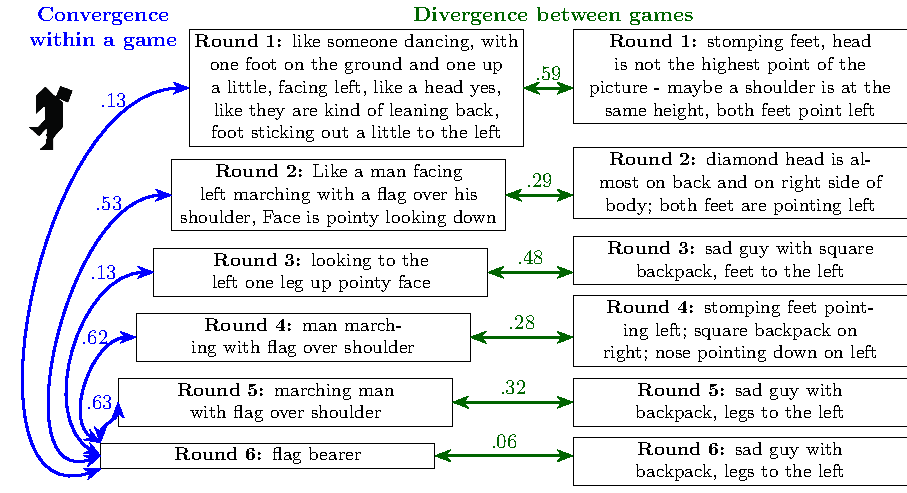
\includegraphics[width=1\linewidth]{sbert} 

}

\caption{Example utterances describing the shown tangram figure produced by two 3-player games in Experiment 1. To measure convergence within a game (blue), we measured the cosine similarity between SBERT embeddings of descriptions and the embedding of the round 6 utterance (taken to be the convention). Higher cosine similarity indicates more similar meaning. To measure divergence between games (green), we measured the similarity between embeddings of utterances from the same round across games.}\label{fig:sbert-diagram}
\end{figure*}

In the previous sections, we examined three metrics of communicative performance in groups of different sizes and interaction structures.
We confirmed that groups in all conditions replicated the classic patterns of increasing accuracy and decreasing description length.
We also found some initial evidence that larger groups may struggle to improve performance in the absence of thick communication channels.
Here, we aim to better understand the mechanisms that allow describers to use shorter descriptions without sacrificing accuracy.
In particular, we explore the hypothesis that interaction structure and group size affect performance through a \emph{convention formation} process (\protect\hyperlink{ref-clark1986}{Clark \& Wilkes-Gibbs 1986}).
Under a recent model of convention formation (\protect\hyperlink{ref-hawkins2023partners}{Hawkins et al. 2023}), groups are able to leverage their shared history to coordinate on stable expectations about how to refer to particular images.
This model makes specific predictions about how interaction structure affects the ability to coordinate, in terms of the available feedback.

First, due to heterogeneity in the group -- 6 individuals who may have diverging conceptualizations --- a rational describer should provide a strictly more detailed initial description to hedge against multiple possible misunderstandings, as we previously observed.
Second, all groups should display the characteristic dynamics of conventions: \emph{stability}, or convergence within group, and \emph{arbitrariness}, or divergence to multiple equilibria across groups.
Third, convergence should be faster when a single individual is consistently in the describer role and when matchers are able to freely respond in natural language, as describers are able to aggregate feedback about the effectiveness of their own utterances from block to block and also immediately correct specific misunderstandings within a given trial.

To assess the dynamics of describer descriptions, we examine the \emph{semantic similarity} of descriptions within and across games.
We quantified description similarity by concatenating describer messages together within a trial and embedding this description into a high-dimensional vector space using SBERT.
SBERT is a BERT-based sentence embedder designed to map semantically similar sentences to embeddings that are nearby in embedding space.
Semantically meaningful comparisons between sentences are made by taking pairwise cosine similarities between the embeddings (\protect\hyperlink{ref-reimers2019}{Reimers \& Gurevych 2019}).

To measure stability, or convergence within groups, we compared utterances from blocks one through five to the final (block six) description for the same image from the same game.
To measure arbitrariness, or divergence across groups depending on group-specific history, we compared utterances produced by different describers for the same image in the corresponding blocks.
Figure \ref{fig:sbert-diagram} illustrates these two measures with example utterances and their within-game and between-game cosine similarities.

\begin{figure*}[t!]

{\centering \includegraphics[width=1\linewidth]{figs/sbert-1} 

}

\caption{Language similarity results measured with pairwise cosine similarity between embeddings of two utterances. (A-C). Convergence of descriptions within games as measured by similarity between an utterance from block 1-5 to the block 6 utterance in the same game for the same image. (D-F). Divergence of descriptions across games as measured by the similarity between two utterances produced for the same image by different groups in the same block. For all, small dots are per game, per block means, and smooth lines are predictions from model fixed effects with 95\% credible intervals. Y-axes are truncated, and a few outliers points are not visible.}\label{fig:sbert}
\end{figure*}

We modeled semantic convergence with a mixed effects linear regression model predicting the similarity between a block 1-5 utterance and the corresponding block 6 utterance as a function of the earlier block number and condition (Figure \ref{fig:sbert}A-C; SI Tables 23-27).
All conditions showed some convergence toward a conventional ``shorthand'' for the picture, but the speed of convergence was affected both by group size and channel width.
First, we found that smaller groups reached stable descriptions faster than larger games.
In Experiment 1, initial similarity was invariant across group size (\(\beta=-0.008,\:95\%\:\mathrm{CrI}=[-0.021, 0.005]\)), but smaller groups converged faster (Figure \ref{fig:sbert}A, \(\beta=-0.008,\:95\%\:\mathrm{CrI}=[-0.011, -0.005]\)).
In Experiment 3, 6-person thick games started off further from their eventual convention than 2-person thick games (\(\beta=-0.069,\:95\%\:\mathrm{CrI}=[-0.113, -0.025]\)) but closed the gap over time (Figure \ref{fig:sbert}C, \(\beta=0.009,\:95\%\:\mathrm{CrI}=[0.001, 0.017]\)).
Second, thicker games tended to converge faster than thin games (Figure \ref{fig:sbert}B-C).
In Experiment 3, small thin games started off slightly further from their convention than small thick games, and this gap widened over time (\(\beta=-0.025,\:95\%\:\mathrm{CrI}=[-0.033, -0.017]\)).
Finally, the combination of thin interaction structure and larger group hindered convergence more than either factor individually.
Beyond the generally slower convergence in thin games, 6-person thin games showed substantially slower convergence even compared to 2-person thin games in Experiment 3 (\(\beta=-0.035,\:95\%\:\mathrm{CrI}=[-0.047, -0.025]\)).

Pooling across experiments in a mega-analysis confirms this pattern.
Thin games converge less than thick games overall (\(\beta=-0.016,\:95\%\:\mathrm{CrI}=[-0.025, -0.008]\)), and \emph{large} thin games are especially slow to converge (\(\beta=-0.007,\:95\%\:\mathrm{CrI}=[-0.01, -0.004]\)).
Across games, convergence towards the last utterance was driven by cumulative increasing similarity between pairs of utterances in adjacent blocks (Supplement Figure 5D-F, SI Tables 38-42).
In early rounds, descriptions could change substantially between rounds, but by later rounds, many descriptions had already reduced and solidified and varied little round to round.
In summary, we found that stable descriptions emerged earlier if the group was smaller, or if the group had a thick interaction structure.

\hypertarget{games-with-thicker-channels-diverge-from-one-another-more-quickly}{%
\subsubsection{Games with thicker channels diverge from one another more quickly}\label{games-with-thicker-channels-diverge-from-one-another-more-quickly}}

While groups may initially overlap in their descriptions, including details of shapes or body parts, we predicted that their descriptions would become increasingly dissimilar as groups increasingly adapt to their own idiosyncratic shared history.
To test this effect, we constructed a mixed-effects linear regression model predicting the cross-game similarity between a pair of utterances for the same image.
A decrease in the similarity between different groups descriptions occurred in every condition, indicating increasing arbitrariness and group-specificity of descriptions (Figure \ref{fig:sbert}D-F, SI Tables 28-32).
However, different game sizes and interaction structures revealed very different strengths of divergence.

First, smaller games used more group-specific language.
In Experiment 1, smaller games diverged more quickly than larger games (\(\beta=0.001,\:95\%\:\mathrm{CrI}=[0.001, 0.002]\)).
In Experiment 3, 2-person thick games started off more dissimiliar than 6-person thick games, although 6-person games diverged faster and eventually approached the dissimilarity levels of 2-person thick games (SI Table 32).
Second, thicker interaction structure was associated with stronger group-specific divergence.
In Experiment 3, 2-person thin games diverged more slowly than 2-person thick games (\(\beta=0.004,\:95\%\:\mathrm{CrI}=[0.002, 0.005]\)).
As with the convergence patterns, large games with thin interaction structures had the flattest trajectories, as thinness and largeness compounded.
In Experiment 3, 6-person thin games diverged even less than 2-player thin games (Figure \ref{fig:sbert}F, \(\beta=0.017,\:95\%\:\mathrm{CrI}=[0.015, 0.019]\)), and in Experiment 2, 6-person thin games barely diverged at all (Figure \ref{fig:sbert}E, \(\beta=-0.004,\:95\%\:\mathrm{CrI}=[-0.006, -0.001]\)).
A mega-analytic model confirms this pattern: thin games differentiate less between groups (\(\beta=0.005,\:95\%\:\mathrm{CrI}=[0.004, 0.007]\)) and large thin groups differentiate even less (\(\beta=0.004,\:95\%\:\mathrm{CrI}=[0.004, 0.005]\)).

\hypertarget{general-discussion}{%
\section{General Discussion}\label{general-discussion}}

Communication often occurs in multi-party settings, but research on referential communication typically does not focus on such settings -- largely due to practical obstacles.
Dyadic reference games have been used to measure informational efficiency, characterized by describer-matcher pairs creating conventional (stable but somewhat arbitrary) labels which are not shared by other groups.
In the current work, we asked how this process of reference formation unfolds in larger groups and under varying interaction structures.
Across 3 online experiments and 11 experimental conditions, we varied game features including group size, form of matcher backchannel, and degree of group coherence.
All conditions replicated classic phenomena: increasing accuracy, reduction in describer utterances, semantic convergence within games, and differentiation of descriptions between groups.
However, we also found that the interaction structure of a group substantially affects how rapidly groups develop partner-specific conventions.
Small groups may be able to form conventions under limited feedback, but larger groups require thicker interaction structure.
Multi-player groups may therefore reveal key factors which are masked in purely dyadic settings.

Increasing efficiency has often been taken as an index of group-specific convention formation (\protect\hyperlink{ref-clark1986}{Clark \& Wilkes-Gibbs 1986}, \protect\hyperlink{ref-brennan1996}{Brennan \& Clark 1996}, \protect\hyperlink{ref-yoon2014}{Yoon \& Brown-Schmidt 2014}, \protect\hyperlink{ref-yoon2018}{2018}).
In our work, however, we observe distinct patterns for measures of raw utterance length compared to the dynamics of semantic content.
In Experiment 3, thin 6-person games showed much less group-specific divergence despite comparable accuracy and efficiency.
This gap raises the possibility that it is possible to become more efficient and accurate without converging on a unified group-specific label.
Instead, they may be converging to a multi-label solution based on group priors (\protect\hyperlink{ref-guilbeault2021}{Guilbeault et al. 2021}).
Thus, we encourage measures of semantic content (and not just performance) when evaluating convention formation.

Even within the general framework of iterated reference, there is a high dimensional feature space of possible experiments. We sampled only a few points along a few dimensions in the space that felt salient. In our experiment 3, we grouped some factors together in order to have more games in each condition: a fully factorial design would have been too expensive to power adequately. We instantiated a ``thin'' channel by limited matchers to 4 discrete utterances (emojis), but there are other ways to manipulate channel width for describers and matchers, such as rate limiting typing or adding time pressure. Future work could sample other points in the experimental space, including exploring other manipulations on channel thickness, the effects of different target images, or groups of people with real-life prior connections.

We cannot make causal claims about specific mechanisms by which manipulations such as group size resulted in different outcomes: there are many differences between being in a 2-person group versus a 6-person group that could lead to the different outcomes. In a dyad, producers can tailor their utterances to the one matcher, but in large groups, producers must balance the competing needs of different comprehenders (\protect\hyperlink{ref-schober1989}{Schober \& Clark 1989}, \protect\hyperlink{ref-tolins2016}{Tolins \& Fox Tree 2016}). These effects likely vary by both the knowledge state of and communication channels available to the comprehenders (\protect\hyperlink{ref-horton2002}{Horton \& Gerrig 2002}, \protect\hyperlink{ref-horton2005}{Horton \& Gerrig 2005}, \protect\hyperlink{ref-fox-tree2013}{Fox Tree \& Clark 2013}). Further work digging into the language used and the interactions between participants might unearth plausible mechanisms for how differences in group size and interaction structure influence outcomes, and this in turn could then point towards future experimental conditions.

Communication occurs across a broad range of situations, varying on many dimensions, including group size, medium of interaction, and group structure.
A narrow focus on dyads with rich communication channels can lead to theories that mispredict how interactions play out in multi-party groups with varying interaction structure.
Sampling from a broader range of communicative situations is thus a critical part of better understanding human communication.

\hypertarget{methods}{%
\section{Methods}\label{methods}}

Our iterated reference task was implemented with Empirica (\protect\hyperlink{ref-almaatouq2020empirica}{Almaatouq et al. 2021}), a React-based web development framework for real-time multi-player tasks.
Our experiments were designed sequentially and pre-registered individually.\footnote{Experiment 1: \url{https://osf.io/cn9f4} for the 2-4 player groups, and \url{https://osf.io/rpz67} for the 5-6 player data run later. Experiment 2: same describer at \url{https://osf.io/f9xyd}, full feedback at \url{https://osf.io/j5zbm}, and thin at \url{https://osf.io/k5f4t}. Experiment 3: \url{https://osf.io/untzy}}
We followed the pre-registered analysis plan for each experiment, although accuracy models were not explicitly specified until Experiment 3, and linguistic analyses were only verbally described starting with Experiment 2b.
Results from some pre-registered models are omitted from the main text for brevity but are shown in the Supplement.
Exploratory mega-analytic models pooling across the three experiments were not pre-registered.

\hypertarget{participants}{%
\subsubsection{Participants}\label{participants}}

Participants were recruited using the Prolific platform.
All participants self-reported as fluent native English speakers on Prolific's demographic prescreen.
Experiment 1 took place between May and July 2021, Experiment 2 between March and August 2022, and Experiment 3 in October 2022.
Each participant took part in only one experiment and was blocked from participating in subsequent experiments.
As games with more participants tended to run longer, we paid participants different rates based on group size, with the goal of a consistent \$10 hourly rate. Participants were paid \$7 for 2-player games, \$8.50 for 3-player games, \$10 for 4-player games, and \$11 for 5- and 6-player games. When one player occupied the describer role for the entirety of a 6-player game, they were rewarded an additional \$2 bonus. Across all games, participants could earn up to \$2.88 in performance bonuses. A total of 1319 people participated across the 3 experiments, for roughly 20 games in each condition in experiments 1 and 2 and 40 games per condition in experiment 3. A breakdown of number of games and participants in each condition is shown in SI Table 3.

\hypertarget{materials}{%
\subsubsection{Materials}\label{materials}}

The same 12 tangram images, drawn from Hawkins et al. (\protect\hyperlink{ref-hawkins2020}{2020}) and Clark \& Wilkes-Gibbs (\protect\hyperlink{ref-clark1986}{1986}), were used every block.
These images were displayed in a 4 \(\times\) 3 grid with the order randomized across participants to disincentivize spatial descriptions such as ``top left,'' as the image might be in a different place on the describer's and matchers' screens.
To reduce cognitive load from visual search, the locations were fixed for each participant across trials.

\hypertarget{procedure}{%
\subsubsection{Procedure}\label{procedure}}

The experimental procedure was very similar across the three experiments.
We first describe the procedure used in Experiment 1 and then describe the differences in later experiments.

\paragraph{Experiment 1}

Participants were directed from Prolific to our custom web application, where they were presented with a consent form and a series of instruction pages explaining the protocol.
After finishing the instructions, they needed to pass a quiz to proceed.
They were then directed to a ``waiting room'' lobby.
Once the lobby filled to the required number of players, the game began. One lobby was filled before another was started; if a participant was waiting for 5 minutes, that lobby timed out, and the participant was paid without completing the experiment. Due to technical constraints with assigning participants to lobbies and games, only games of a single experimental condition could be active at a time. Thus, different conditions were run on different days or times of day.\\
One of the participants was randomly selected to begin in the role of describer, and the other participants were assigned to the role of matchers.
On each trial, the describer saw a fixed array of tangrams with one tangram (privately) highlighted as the \emph{target}.
They were given a chat interface to communicate the target to the matchers, who were asked to determine which of the 12 images was the referential target.
All participants were free to use the chat box to communicate at any time, but matchers could only make a selection after the describer had sent a message.
Once a matcher clicked, they could not change their selection.
There was no signal to the describer or other matchers about who had already made a selection.
We recorded what all participants said in the chat, as well as who selected which image and how long they took to make their selections.

Once all matchers had made a selection (or a 3-minute timer ran out), participants were given feedback and proceeded to the next trial.
Matchers only received \emph{binary} feedback about whether they had chosen correctly or not; that is, matchers who made an incorrect choice were not shown the correct answer (see Supplement Figure 1 for example feedback).
The describer saw which tangram each matcher selected, but matchers did not see one another's selections.
Matchers got 4 points for each correct answer; the describer got points equal to the average of the matchers' points.
These points were translated into performance bonuses at the end of the experiment (1 point = 1 cent bonus).
After the describer had described each of the 12 images as targets, in a randomized sequence, the process repeated with the same set of targets, for a total of 6 such repetition blocks (72 trials).

The same person was the describer for an entire block, but participants rotated roles between blocks.
Thus, over the course of the 6 blocks, participants were describers 3 times in 2-player games, twice in 3-player games, once or twice in 4 and 5-player games, and once in 6-player games.
Rotating the describer was chosen in this first experiment to keep participants more equally engaged (the describer role is more work), and to provide a more robust test of our hypotheses regarding efficiency and convention formation.
After the game finished, participants were given a survey asking for optional demographic information and feedback on their experience with the game.

If a participant disconnected from the experiment, the game would stop.

\paragraph{Experiment 2}

Experiment 2 consisted of three different variations on Experiment 1, all conducted in 6-player games.
Each of these conditions differed from the Experiment 1 baseline in exactly one way.
In the \emph{same describer} condition, one person was designated the describer for the entire game, rather than having the describer role rotate.
In the \emph{full feedback} condition, all participants were shown what all others had selected as well as the identity of the correct target.
This condition was similar to previous dyadic work, such as Hawkins et al. (\protect\hyperlink{ref-hawkins2020}{2020}), where the correct answer was indicated during feedback.
In the \emph{thin} condition, we altered the chatbox interface for matchers.
Instead of a textbox, matchers had 4 buttons, each of which sent a different emoji to the chat. Matchers were given suggested meanings for the 4 emojis during the instruction phase. They could send as many emojis as desired; for instance, they might initially indicate confusion, and later indicate understanding. In addition, for the thin condition, we added notifications that appeared in the chat box marking the time when each player had made a selection.

\paragraph{Experiment 3}

The thin channel condition in Experiment 3 was the same as the thin condition in Experiment 2.
The thick condition combined the two coherency-enhancing variations from Experiment 2: the same participant remained in the describer role throughout, and full feedback was given about the correct answer and what all other players had selected.
Across both conditions in Experiment 3, notifications were sent to the chat to indicate when a participant had made a selection.
For experiment 3, game lobbies worked slightly differently, and 5 minutes after the first participant had joined the lobby, the game started if there were at least two participants. Correspondingly, in experiment 3, games did not stop if a player disconnected, instead if there were at least two players still active, the game continued, swapping a player into the role of describer if necessary to continue the game.

\hypertarget{data-pre-processing-and-exclusions}{%
\subsubsection{Data pre-processing and exclusions}\label{data-pre-processing-and-exclusions}}

Participants could use the chat box freely, which meant that the chat transcript contained some non-referential language. The first author skimmed the chat transcripts, tagging utterances that did not refer to the current tangram. These were primarily pleasantries (``Hello''), meta-commentary about how well the task was going, and bare confirmations or denials (``ok'', ``got it'', ``yes'', ``no''). We excluded these utterances from our analyses. Note that chat lines sometimes included non-referential words in addition to words referring to the tangrams (``ok, so it looks like a zombie'', ``yes, the one with legs''); these lines were retained intact.

In Experiments 1 and 2, games did not start if there were not enough participants and ended if any participant disconnected.
In Experiment 3, games started after a waiting period even if they were not entirely full and continued even in the event that a participant disconnected (with describer role reassigned if necessary), unless the game dropped below 2 players.
The distribution of player counts in games that were initially recruited to be 6 player games is shown in SI Figure 2.
The realities of online recruitment and disconnection meant that the number of games varied between conditions.
We excluded incomplete blocks from analyses, but included complete blocks from partial games (See SI Table 3).
When skimming transcripts to tag non-referential utterances, we noticed that one game in the 6-player thick condition had a describer who did not give any sort of coherent descriptions, even with substantial matcher prompting. We excluded this game from analyses.

\hypertarget{modelling-strategy}{%
\subsubsection{Modelling strategy}\label{modelling-strategy}}

We fit all regression models in brms (\protect\hyperlink{ref-burkner2018}{Bürkner 2018}) with weakly regularizing priors.
We were unable to fit the full pre-registered mixed effects structure in a reasonable amount of time for some models, so we included the maximal hierarchical effects that were tractable.
All model results and priors and formulae are reported in the Supplement.
Models of accuracy used by-group random intercepts only, models of word count used full mixed effect structure, and models of S-BERT similarities used by-group and by-target random intercepts as applicable.
Models of matcher accuracy were logistic models with normal(0,1) priors for betas and sd.
Models of describer efficiency were run as linear models with an intercept prior of normal(12,20), a beta prior of normal(0,10), an sd prior of normal(0,5) and a random-effect correlation prior of lkj(1).
For all of the models of SBERT similarity, we used linear models with the priors normal(.5,.2) for the intercept, normal(0,.1) for betas, and normal(0,.05) for sd.
As an additional post-hoc analysis, we ran mega-analytic models combining data across all experiments.
For these models, we grouped the 3 thin-ish conditions (2c, and the two thin conditions of experiment 3) as one level, and coded the rest of the conditions as thick-ish.
Game size was coded as a continuous measure (2 through 6). The priors for the mega-analytic models were the same as for the per-experiment models described above.

We also needed to decide how to handle dropout in Experiment 3, as some of the 6-player games did not retain all 6 players for the entire game.
Our decision was to follow an intent-to-treat analysis and treat data as missing completely at random.
Note that this choice underestimates differences between 2-player and (genuine) 6-player games by labeling some smaller groups as 6-player groups.
We do not know exactly what leads some participants to drop out, but it is possible that some factors may be random (ex. connection issues) and others may be correlated with performance (ex. frustration because group is struggling).\\
We do not know whether groups that start and continue at the full size differ from games where some participants drop out.
This is potentially an issue across all experiments; in experiments 1 and 2, groups stopped playing if anyone dropped out, and in experiment 3 they kept playing as a smaller group.
The number of games in each condition and rates of dropoff are shown in SI Table 3 and SI Figure 2.

\hypertarget{authors-note}{%
\section{Author's Note}\label{authors-note}}

Experiment 1 was previously reported in Proceedings of the Annual Meeting of the Cognitive Science Society 44 (2022).

We thank the LangCog Lab, Saxelab, CAMP 5, HSP 2023, and Cogsci 2022 audiences for helpful feedback on this work. This work was supported by a Hoffman-Yee Grant from the Stanford Institute for Human-Centered AI.

We report CRediT taxonomy contributions as follows: All authors did conceptualization and methodology. VB did data curation, formal analysis, investigation, visualization, and writing -- original draft. VB and RDH did software. RDH, NDG, and MCF did writing -- editing. MCF and NDG did funding. MCF did supervision.

\hypertarget{references}{%
\section{References}\label{references}}

\setlength{\parindent}{-0.1in} 
\setlength{\leftskip}{0.125in}

\noindent

\hypertarget{refs}{}
\begin{CSLReferences}{1}{0}
\leavevmode\vadjust pre{\hypertarget{ref-ahern1994effect}{}}%
Ahern TC (1994) The effect of interface on the structure of interaction in computer-mediated small-group discussion. \emph{Journal of Educational Computing Research} \textbf{11}:235--250

\leavevmode\vadjust pre{\hypertarget{ref-almaatouq2020empirica}{}}%
Almaatouq A, Becker J, Houghton JP, Paton N, Watts DJ, Whiting ME (2021) Empirica: A virtual lab for high-throughput macro-level experiments. \emph{Behavior Research Methods} \textbf{53}:2158--2171

\leavevmode\vadjust pre{\hypertarget{ref-almaatouq2022}{}}%
Almaatouq A, Griffiths TL, Suchow JW, Whiting ME, Evans J, Watts DJ (2022) Beyond {Playing} 20 {Questions} with {Nature}: {Integrative Experiment Design} in the {Social} and {Behavioral Sciences}. \emph{Behavioral and Brain Sciences}:1--55. doi:\href{https://doi.org/10.1017/S0140525X22002874}{10.1017/S0140525X22002874}

\leavevmode\vadjust pre{\hypertarget{ref-branigan2006}{}}%
Branigan H (2006) Perspectives on multi-party dialogue. \emph{Research on Language and Computation} \textbf{4}:153--177

\leavevmode\vadjust pre{\hypertarget{ref-brennan1996}{}}%
Brennan SE, Clark HH (1996) Conceptual {Pacts} and {Lexical Choice} in {Conversation}. :12

\leavevmode\vadjust pre{\hypertarget{ref-burkner2018}{}}%
Bürkner P-C (2018) Advanced bayesian multilevel modeling with the r package brms. \emph{The R Journal} \textbf{10}:395--411

\leavevmode\vadjust pre{\hypertarget{ref-caplow1957organizational}{}}%
Caplow T (1957) Organizational size. \emph{Administrative Science Quarterly}:484--505

\leavevmode\vadjust pre{\hypertarget{ref-carletta1998}{}}%
Carletta J, Garrod S, Fraser-Krauss H (1998) Placement of {Authority} and {Communication Patterns} in {Workplace Groups}: {The Consequences} for {Innovation}. \emph{Small Group Research} \textbf{29}:531--559. doi:\href{https://doi.org/10.1177/1046496498295001}{10.1177/1046496498295001}

\leavevmode\vadjust pre{\hypertarget{ref-cazden1988classroom}{}}%
Cazden CB (1988) Classroom discourse: The language of teaching and learning. ERIC

\leavevmode\vadjust pre{\hypertarget{ref-clark2004speaking}{}}%
Clark HH, Krych MA (2004) Speaking while monitoring addressees for understanding. \emph{Journal of memory and language} \textbf{50}:62--81

\leavevmode\vadjust pre{\hypertarget{ref-clark1986}{}}%
Clark HH, Wilkes-Gibbs D (1986) \href{http://www.speech.kth.se/~edlund/bielefeld/references/clark-and-wilkes-gibbs-1986.pdf}{Referring as a collaborative process}. \emph{Cognition}

\leavevmode\vadjust pre{\hypertarget{ref-cohngordon}{}}%
Cohn-Gordon Reuben, Levy R, Bergen L (2019) The pragmatics of multiparty communication.

\leavevmode\vadjust pre{\hypertarget{ref-dewhirst1971influence}{}}%
Dewhirst HD (1971) Influence of perceived information-sharing norms on communication channel utilization. \emph{Academy of Management Journal} \textbf{14}:305--315

\leavevmode\vadjust pre{\hypertarget{ref-fay2000}{}}%
Fay N, Garrod S, Carletta J (2000) Group {Discussion} as {Interactive Dialogue} or as {Serial Monologue}: {The Influence} of {Group Size}. \emph{Psychol Sci} \textbf{11}:481--486. doi:\href{https://doi.org/10.1111/1467-9280.00292}{10.1111/1467-9280.00292}

\leavevmode\vadjust pre{\hypertarget{ref-fox-tree2013}{}}%
Fox Tree JE, Clark NB (2013) Communicative {Effectiveness} of {Written Versus Spoken Feedback}. \emph{Discourse Processes} \textbf{50}:339--359. doi:\href{https://doi.org/10.1080/0163853X.2013.797241}{10.1080/0163853X.2013.797241}

\leavevmode\vadjust pre{\hypertarget{ref-garrod2007foundations}{}}%
Garrod S, Fay N, Lee J, Oberlander J, MacLeod T (2007) Foundations of representation: Where might graphical symbol systems come from? \emph{Cognitive science} \textbf{31}:961--987

\leavevmode\vadjust pre{\hypertarget{ref-ginzburg2005}{}}%
Ginzburg J, Fernandez R (2005) Action at a distance: The difference between dialogue and multilogue. \emph{Proceedings of DIALOR}:9

\leavevmode\vadjust pre{\hypertarget{ref-guilbeault2021}{}}%
Guilbeault D, Baronchelli A, Centola D (2021) Experimental evidence for scale-induced category convergence across populations. \emph{Nat Commun} \textbf{12}:327. doi:\href{https://doi.org/10.1038/s41467-020-20037-y}{10.1038/s41467-020-20037-y}

\leavevmode\vadjust pre{\hypertarget{ref-haber2019}{}}%
Haber J, Baumgärtner T, Takmaz E, Gelderloos L, Bruni E, Fernández R (2019) The {PhotoBook Dataset}: {Building Common Ground} through {Visually-Grounded Dialogue}. In: \emph{Proc. 57th {Annu}. {Meet}. {Assoc}. {Comput}. {Linguist}.} {Association for Computational Linguistics}, {Florence, Italy}, p 1895--1910. Available from: \url{https://www.aclweb.org/anthology/P19-1184} {[}Last accessed 1 February 2022{]}. doi:\href{https://doi.org/10.18653/v1/P19-1184}{10.18653/v1/P19-1184}

\leavevmode\vadjust pre{\hypertarget{ref-hawkins2020}{}}%
Hawkins RD, Frank MC, Goodman ND (2020) \href{http://arxiv.org/abs/1912.07199}{Characterizing the dynamics of learning in repeated reference games}. \emph{ArXiv191207199 Cs}

\leavevmode\vadjust pre{\hypertarget{ref-hawkins2023partners}{}}%
Hawkins RD, Franke M, Frank MC, Goldberg AE, Smith K, Griffiths TL, Goodman ND (2023) From partners to populations: A hierarchical bayesian account of coordination and convention. \emph{Psychological Review} \textbf{130}:977

\leavevmode\vadjust pre{\hypertarget{ref-hiltz1986experiments}{}}%
Hiltz SR, Johnson K, Turoff M (1986) Experiments in group decision making: Communication process and outcome in face-to-face versus computerized conferences. \emph{Human communication research} \textbf{13}:225--252

\leavevmode\vadjust pre{\hypertarget{ref-horton2002}{}}%
Horton WS, Gerrig RJ (2002) {SpeakersÕ} experiences and audience design: Knowing when and knowing how to adjust utterances to addresseesq. \emph{Journal of Memory and Language}:18

\leavevmode\vadjust pre{\hypertarget{ref-horton2005}{}}%
Horton WS, Gerrig RJ (2005) The impact of memory demands on audience design during language production. \emph{Cognition} \textbf{96}:127--142. doi:\href{https://doi.org/10.1016/j.cognition.2004.07.001}{10.1016/j.cognition.2004.07.001}

\leavevmode\vadjust pre{\hypertarget{ref-ji2022abstract}{}}%
Ji A, Kojima N, Rush N, Suhr A, Vong WK, Hawkins R, Artzi Y (2022) Abstract visual reasoning with tangram shapes. In: \emph{Proceedings of the 2022 conference on empirical methods in natural language processing}.p 582--601

\leavevmode\vadjust pre{\hypertarget{ref-KraussBricker67_Delay}{}}%
Krauss RM, Bricker PD (1967) Effects of transmission delay and access delay on the efficiency of verbal communication. \emph{The Journal of the Acoustical Society of America} \textbf{41}:286--292

\leavevmode\vadjust pre{\hypertarget{ref-krauss1964}{}}%
Krauss RM, Weinheimer S (1964) Changes in reference phrases as a function of frequency of usage in social interaction: A preliminary study. \emph{Psychon Sci} \textbf{1}:113--114. doi:\href{https://doi.org/10.3758/BF03342817}{10.3758/BF03342817}

\leavevmode\vadjust pre{\hypertarget{ref-krauss1966}{}}%
Krauss RM, Weinheimer S (1966) Concurrent feedback, confirmation, and the encoding of referents in verbal communication. \emph{Journal of Personality and Social Psychology} \textbf{4}:343--346. doi:\href{https://doi.org/10.1037/h0023705}{10.1037/h0023705}

\leavevmode\vadjust pre{\hypertarget{ref-KraussEtAl77}{}}%
Krauss RM, Garlock CM, Bricker PD, McMahon LE (1977) The role of audible and visible back-channel responses in interpersonal communication. \emph{Journal of Personality and Social Psychology} \textbf{35}:523

\leavevmode\vadjust pre{\hypertarget{ref-kraut1982listener}{}}%
Kraut RE, Lewis SH, Swezey LW (1982) Listener responsiveness and the coordination of conversation. \emph{Journal of personality and social psychology} \textbf{43}:718

\leavevmode\vadjust pre{\hypertarget{ref-lewis1969convention}{}}%
Lewis D (1969) Convention: A philosophical study. John Wiley \& Sons

\leavevmode\vadjust pre{\hypertarget{ref-macmillan_communication_2004}{}}%
MacMillan J, Entin EE, Serfaty D (2004) Communication overhead: {The} hidden cost of team cognition. In: \emph{Team cognition: {Understanding} the factors that drive process and performance.} American Psychological Association, Washington, DC, US, p 61--82. doi:\href{https://doi.org/10.1037/10690-004}{10.1037/10690-004}

\leavevmode\vadjust pre{\hypertarget{ref-metzing2003}{}}%
Metzing C, Brennan SE (2003) When conceptual pacts are broken: {Partner-specific} effects on the comprehension of referring expressions. \emph{Journal of Memory and Language} \textbf{49}:201--213. doi:\href{https://doi.org/10.1016/S0749-596X(03)00028-7}{10.1016/S0749-596X(03)00028-7}

\leavevmode\vadjust pre{\hypertarget{ref-parisi2005evaluating}{}}%
Parisi JA, Brungart DS (2005) Evaluating communication effectiveness in team collaboration. In: \emph{Ninth european conference on speech communication and technology (INTERSPEECH)}.

\leavevmode\vadjust pre{\hypertarget{ref-reimers2019}{}}%
Reimers N, Gurevych I (2019) Sentence-{BERT}: {Sentence Embeddings} using {Siamese BERT-Networks}. doi:\href{https://doi.org/10.48550/arXiv.1908.10084}{10.48550/arXiv.1908.10084}

\leavevmode\vadjust pre{\hypertarget{ref-rogers2013}{}}%
Rogers SL, Fay N, Maybery M (2013) Audience {Design} through {Social Interaction} during {Group Discussion}. \emph{PLOS ONE} \textbf{8}:e57211. doi:\href{https://doi.org/10.1371/journal.pone.0057211}{10.1371/journal.pone.0057211}

\leavevmode\vadjust pre{\hypertarget{ref-schober1989}{}}%
Schober MF, Clark HH (1989) Understanding by addressees and overhearers. \emph{Cognitive Psychology} \textbf{21}:211--232. doi:\href{https://doi.org/10.1016/0010-0285(89)90008-X}{10.1016/0010-0285(89)90008-X}

\leavevmode\vadjust pre{\hypertarget{ref-seaman1997communication}{}}%
Seaman CB, Basili VR (1997) Communication and organization in software development: An empirical study. \emph{IBM Systems Journal} \textbf{36}:550--563

\leavevmode\vadjust pre{\hypertarget{ref-swaab2012communication}{}}%
Swaab RI, Galinsky AD, Medvec V, Diermeier DA (2012) The communication orientation model: Explaining the diverse effects of sight, sound, and synchronicity on negotiation and group decision-making outcomes. \emph{Personality and Social Psychology Review} \textbf{16}:25--53

\leavevmode\vadjust pre{\hypertarget{ref-tannen2005conversational}{}}%
Tannen D (2005) Conversational style: Analyzing talk among friends. Oxford University Press

\leavevmode\vadjust pre{\hypertarget{ref-tolins2016}{}}%
Tolins J, Fox Tree JE (2016) Overhearers {Use Addressee Backchannels} in {Dialog Comprehension}. \emph{Cogn Sci} \textbf{40}:1412--1434. doi:\href{https://doi.org/10.1111/cogs.12278}{10.1111/cogs.12278}

\leavevmode\vadjust pre{\hypertarget{ref-traum2004}{}}%
Traum D (2004) Issues in {Multiparty Dialogues}. In: Dignum F (ed) \emph{Advances in {Agent Communication}}. {Springer Berlin Heidelberg}, {Berlin, Heidelberg}, p 201--211. Available from: \url{http://link.springer.com/10.1007/978-3-540-24608-4_12} {[}Last accessed 1 February 2022{]}. doi:\href{https://doi.org/10.1007/978-3-540-24608-4_12}{10.1007/978-3-540-24608-4\_12}

\leavevmode\vadjust pre{\hypertarget{ref-weber2003}{}}%
Weber RA, Camerer CF (2003) Cultural {Conflict} and {Merger Failure}: {An Experimental Approach}. \emph{Manag Sci} \textbf{49}:16

\leavevmode\vadjust pre{\hypertarget{ref-wilkes1992coordinating}{}}%
Wilkes-Gibbs D, Clark HH (1992) Coordinating beliefs in conversation. \emph{Journal of memory and language} \textbf{31}:183--194

\leavevmode\vadjust pre{\hypertarget{ref-Wittgenstein1953}{}}%
Wittgenstein L (1953) Philosophical investigations. Wiley-Blackwell, New York, NY, USA

\leavevmode\vadjust pre{\hypertarget{ref-yoon2014}{}}%
Yoon SO, Brown-Schmidt S (2014) Adjusting conceptual pacts in three-party conversation. \emph{Journal of Experimental Psychology: Learning, Memory, and Cognition} \textbf{40}:919--937. doi:\href{https://doi.org/10.1037/a0036161}{10.1037/a0036161}

\leavevmode\vadjust pre{\hypertarget{ref-yoon2018}{}}%
Yoon SO, Brown-Schmidt S (2018) Aim {Low}: {Mechanisms} of {Audience Design} in {Multiparty Conversation}. \emph{Discourse Processes} \textbf{55}:566--592. doi:\href{https://doi.org/10.1080/0163853X.2017.1286225}{10.1080/0163853X.2017.1286225}

\leavevmode\vadjust pre{\hypertarget{ref-yoon2019}{}}%
Yoon SO, Brown‐Schmidt S (2019) Audience {Design} in {Multiparty Conversation}. \emph{Cogn Sci} \textbf{43}:e12774. doi:\href{https://doi.org/10.1111/cogs.12774}{10.1111/cogs.12774}

\leavevmode\vadjust pre{\hypertarget{ref-zack1993interactivity}{}}%
Zack MH (1993) Interactivity and communication mode choice in ongoing management groups. \emph{Information Systems Research} \textbf{4}:207--239

\end{CSLReferences}


\end{document}
